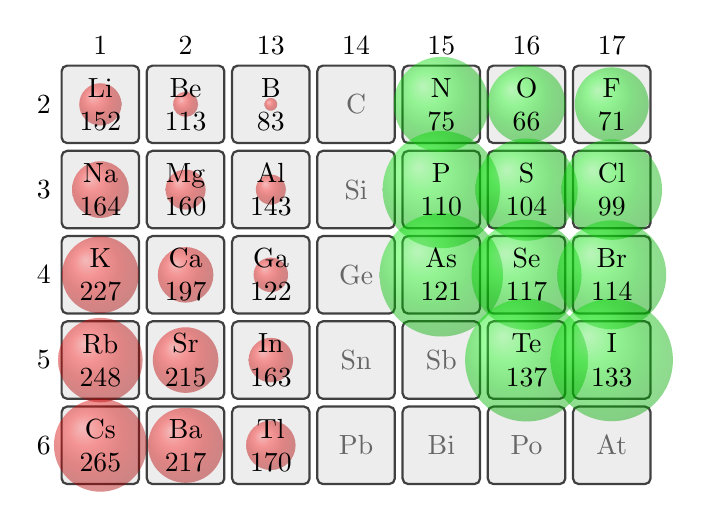
\begin{tikzpicture}
  \def\sep{2pt} % Node distance
  \tikzset
    {
      element/.style = 
        {
          rectangle,
          rounded corners = 2pt,
          thick,
          fill = black!7,
          draw = black!75,
          minimum size = 2.8em,
        },
      atom-radius/.style = 
        {
          nearly transparent, 
          fill = #1,
          ball color = #1,
        },
      cation-radius/.style = { atom-radius = red },
      anion-radius/.style = { atom-radius = green },
    }  

  \begin{scope}[every node/.style = {element}]
    % GRUPO 1
    \node (Li) {};
    \node (Na) [anchor = north, yshift = -\sep] at (Li.south) {};
    \node (K) [anchor = north, yshift = -\sep] at (Na.south) {};
    \node (Rb) [anchor = north, yshift = -\sep] at (K.south) {};
    \node (Cs) [anchor = north, yshift = -\sep] at (Rb.south) {};

    % GRUPO 2
    \node (Be) [anchor = west, xshift = \sep]   at (Li.east) {};
    \node (Mg) [anchor = north, yshift = -\sep] at (Be.south) {};
    \node (Ca) [anchor = north, yshift = -\sep] at (Mg.south) {};
    \node (Sr) [anchor = north, yshift = -\sep] at (Ca.south) {};
    \node (Ba) [anchor = north, yshift = -\sep] at (Sr.south) {};

    % GRUPO 13
    \node (B) [anchor = west, xshift = \sep]    at (Be.east) {};
    \node (Al) [anchor = north, yshift = -\sep] at (B.south) {};
    \node (Ga) [anchor = north, yshift = -\sep] at (Al.south) {};
    \node (In) [anchor = north, yshift = -\sep] at (Ga.south) {};
    \node (Tl) [anchor = north, yshift = -\sep] at (In.south) {};

    % GRUPO 14
    \node (C)  [anchor = west, xshift = \sep]   at (B.east) {};
    \node (Si) [anchor = north, yshift = -\sep] at (C.south) {};
    \node (Ge) [anchor = north, yshift = -\sep] at (Si.south) {};
    \node (Sn) [anchor = north, yshift = -\sep] at (Ge.south) {};
    \node (Pb) [anchor = north, yshift = -\sep] at (Sn.south) {};

    % GRUPO 15
    \node (N)  [anchor = west, xshift = \sep]   at (C.east) {};
    \node (P)  [anchor = north, yshift = -\sep] at (N.south) {};
    \node (As) [anchor = north, yshift = -\sep] at (P.south) {};
    \node (Sb) [anchor = north, yshift = -\sep] at (As.south) {};
    \node (Bi) [anchor = north, yshift = -\sep] at (Sb.south) {};

    % GRUPO 16
    \node (O)  [anchor = west, xshift = \sep]   at (N.east) {};
    \node (S)  [anchor = north, yshift = -\sep] at (O.south) {};
    \node (Se) [anchor = north, yshift = -\sep] at (S.south) {};
    \node (Te) [anchor = north, yshift = -\sep] at (Se.south) {};
    \node (Po) [anchor = north, yshift = -\sep] at (Te.south) {};

    % GRUPO 17
    \node (F)  [anchor = west, xshift = \sep]   at (O.east) {};
    \node (Cl) [anchor = north, yshift = -\sep] at (F.south) {};
    \node (Br) [anchor = north, yshift = -\sep] at (Cl.south) {};
    \node (I)  [anchor = north, yshift = -\sep] at (Br.south) {};
    \node (At) [anchor = north, yshift = -\sep] at (I.south) {};
  \end{scope}

  % RAIOS DOS CÁTIONS
  \fill [cation-radius] (Li) circle (7.6bp);
  \fill [cation-radius] (Na) circle (10.2bp);
  \fill [cation-radius] (K)  circle (13.8bp);
  \fill [cation-radius] (Rb) circle (15.2bp);
  \fill [cation-radius] (Cs) circle (16.7bp);

  \fill [cation-radius] (Be) circle (4.5bp);
  \fill [cation-radius] (Mg) circle (7.2bp);
  \fill [cation-radius] (Ca) circle (10.0bp);
  \fill [cation-radius] (Sr) circle (11.8bp);
  \fill [cation-radius] (Ba) circle (13.5bp);

  \fill [cation-radius] (B)  circle (2.3bp);
  \fill [cation-radius] (Al) circle (5.4bp);
  \fill [cation-radius] (Ga) circle (6.2bp);
  \fill [cation-radius] (In) circle (8.0bp);
  \fill [cation-radius] (Tl) circle (8.9bp);

  % RAIOS DOS ÂNIONS
  \fill [anion-radius] (N)  circle (17.1bp);
  \fill [anion-radius] (P)  circle (21.1bp);
  \fill [anion-radius] (As) circle (22.2bp);

  \fill [anion-radius] (O)  circle (14.0bp);
  \fill [anion-radius] (S)  circle (18.4bp);
  \fill [anion-radius] (Se) circle (19.8bp);
  \fill [anion-radius] (Te) circle (22.1bp);
  
  \fill [anion-radius] (F)  circle (13.3bp);
  \fill [anion-radius] (Cl) circle (18.1bp);
  \fill [anion-radius] (Br) circle (19.6bp);
  \fill [anion-radius] (I)  circle (22.0bp);

  % LABELS GRUPO
  \begin{scope}[anchor = south]
    \node at (Li.north) {1};
    \node at (Be.north) {2};
    \node at (B.north)  {13};
    \node at (C.north)  {14};
    \node at (N.north)  {15};
    \node at (O.north)  {16};
    \node at (F.north)  {17};
  \end{scope}

  % LABELS PERÍODO
  \begin{scope}[anchor = east]
    \node at (Li.west) {2};
    \node at (Na.west) {3};
    \node at (K.west)  {4};
    \node at (Rb.west) {5};
    \node at (Cs.west) {6};
  \end{scope}

  % LABELS ÁTOMOS
  \begin{scope}[align = center]
    \node at (Li) { \ce{Li} \\ \num{152} };
    \node at (Na) { \ce{Na} \\ \num{164} };
    \node at (K)  { \ce{K}  \\ \num{227} };
    \node at (Rb) { \ce{Rb} \\ \num{248} };
    \node at (Cs) { \ce{Cs} \\ \num{265} };

    \node at (Be) { \ce{Be} \\ \num{113} };
    \node at (Mg) { \ce{Mg} \\ \num{160} };
    \node at (Ca) { \ce{Ca} \\ \num{197} };
    \node at (Sr) { \ce{Sr} \\ \num{215} };
    \node at (Ba) { \ce{Ba} \\ \num{217} };

    \node at (B)  { \ce{B}  \\ \num{83} };
    \node at (Al) { \ce{Al} \\ \num{143} };
    \node at (Ga) { \ce{Ga} \\ \num{122} };
    \node at (In) { \ce{In} \\ \num{163} };
    \node at (Tl) { \ce{Tl} \\ \num{170} };

    \node at (N)  { \ce{N}  \\ \num{75} };
    \node at (P)  { \ce{P}  \\ \num{110} };
    \node at (As) { \ce{As} \\ \num{121} };

    \node at (O)  { \ce{O}  \\ \num{66} };
    \node at (S)  { \ce{S}  \\ \num{104} };
    \node at (Se) { \ce{Se} \\ \num{117} };
    \node at (Te) { \ce{Te} \\ \num{137} };
    

    \node at (F)  { \ce{F}  \\ \num{71} };
    \node at (Cl) { \ce{Cl} \\ \num{99} };
    \node at (Br) { \ce{Br} \\ \num{114} };
    \node at (I)  { \ce{I}  \\ \num{133} };
  \end{scope}

  % ÁTOMOS SEM RAIO IÔNICO
  \begin{scope}[black!60]
    \node at (C)  { \ce{C}  };
    \node at (Si) { \ce{Si} };
    \node at (Ge) { \ce{Ge} };
    \node at (Sn) { \ce{Sn} };
    \node at (Pb) { \ce{Pb} };

    \node at (Sb) { \ce{Sb} };
    \node at (Bi) { \ce{Bi} };

    \node at (Po) { \ce{Po} };

    \node at (At) { \ce{At} };
  \end{scope}

\end{tikzpicture}
  
  